\section{Survey Sections} \label{sec:survey}
do survey stuff here

Possible: ``dimensions of assurances''?

\begin{itemize}
    \item intentional/unintentional
    \item atomic/composite
    \item source AIA behavior
    \item target trust variable
    \item methods from \cite{Lacave2002-cu} -- includes numerical information, 80\% success vs. 20\% failure, etc\ldots
\end{itemize}

need to add a lot of material. should have some kind of ``take-away'' graphic or table to summarize the overall findings of the survey.

\subsection{Intentional and Unintentional Assurances}
    There seems to be quite a large disparity of the kinds of assurances studied by the formal and informal trust groups, as depicted in Figure \ref{fig:trust_assurance_intention}.  This is most likely due to the differing interests and skill sets. Those studying unintentional assurances seem to be more interested in investigating the human-AIA relationship. On the other hand those investigating the effect of intentional assurances are more interested in making algorithms.
    
    This figure clearly shows that there is a large space for researchers who study intentional assurances within a formal trust framework. To state the idea more clearly, this would involve actively designing assurances based on the AIA capability, and the assurance classes, and then validating these assurances in designed experiments.

    \textbf{add more stuff \ldots}

	\begin{figure}[htbp]
    	\centering
     	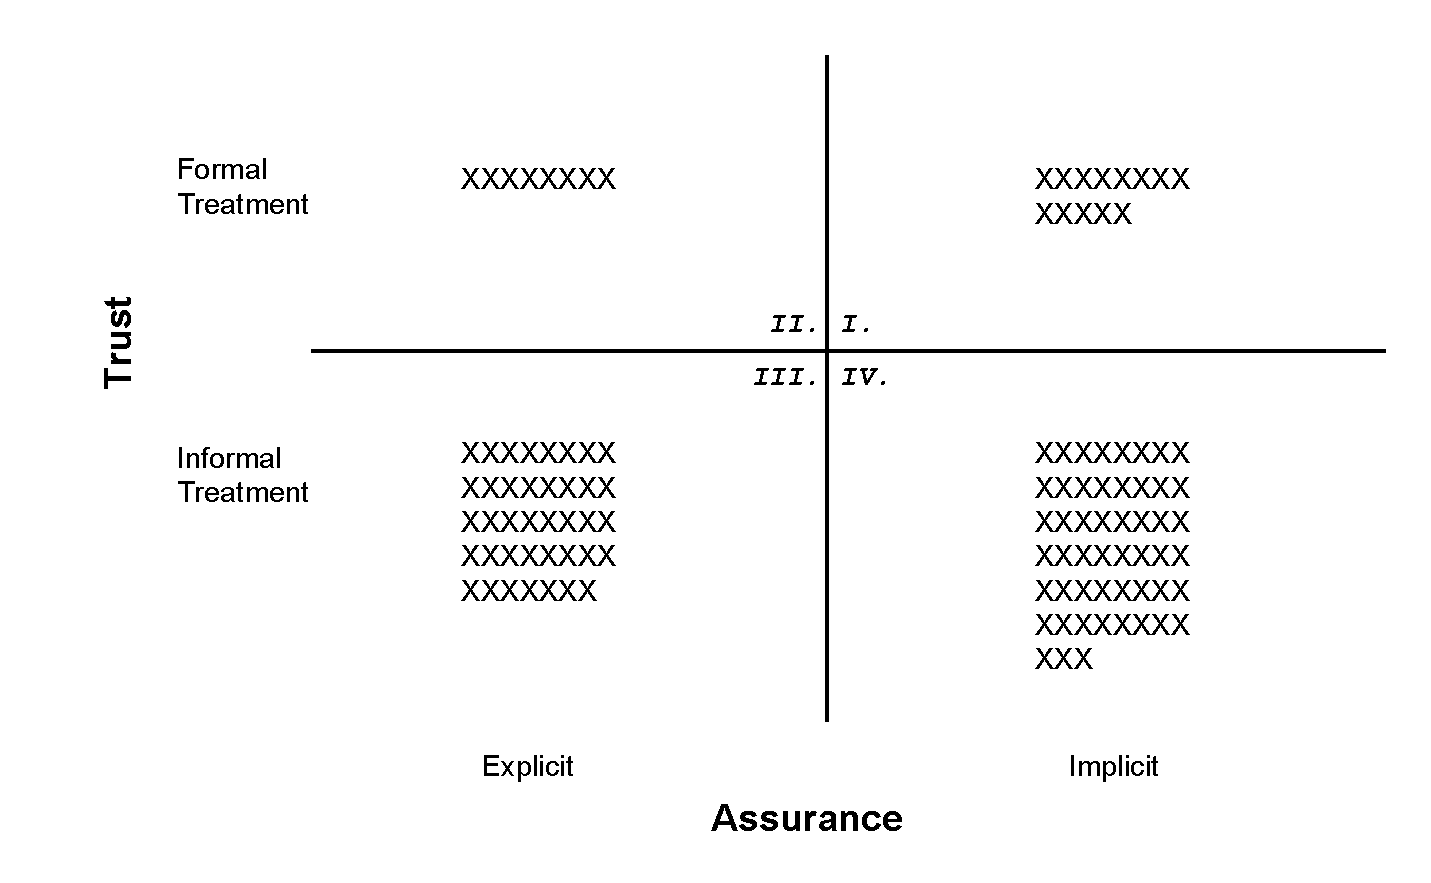
\includegraphics[width=0.6\textwidth]{Figures/Trust_vs_Assurance_Intention.pdf}
    	\caption{Figure depicting how many papers that consider trust formally/informally consider intentional/unintentional assurances, \textbf{need to put actual data here, if it is a useful figure, for now the data is approximate from my memory}}
        \label{fig:trust_assurance_intention}
    \end{figure}

\subsection{Atomic and Composite Assurances}
    Considering the reality that, given the existence of intentional and unintentional assurances, it is unrealistic to assume that, in a practical setting, only atomic assurances exist.

	\begin{figure}[htbp]
    	\centering
     	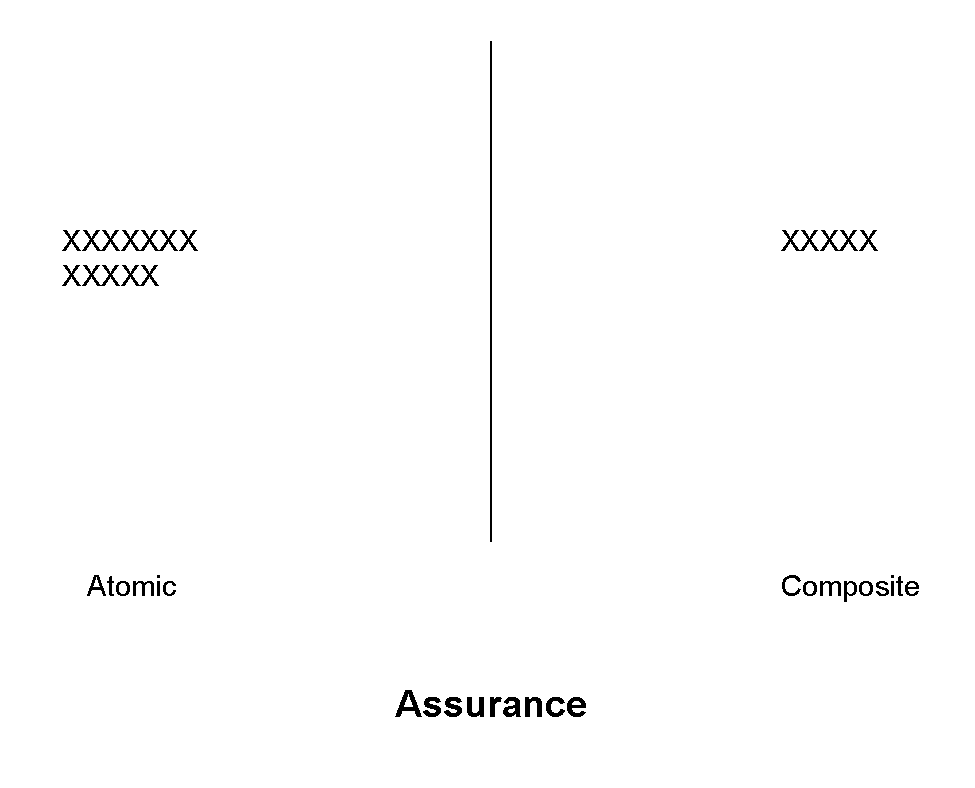
\includegraphics[width=0.5\textwidth]{Figures/Assurances_atomic_composite.pdf}
    	\caption{Figure showing the number of research papers dedicated to composite and atomic assurances}
        \label{fig:trust_assurance_intention}
    \end{figure}


\subsection{Other stuff \ldots}
